\documentclass{article}
\usepackage{amsmath}
\usepackage{graphicx}
\usepackage[utf8]{inputenc}
\newcommand{\myvec}[1]{\ensuremath{\begin{pmatrix}#1\end{pmatrix}}}
\title{Assignment 1}
\author{D V K M Rishab \\ \\ AI20MTECH14004}
\date{}
\begin{document}
\let\vec\mathbf
\maketitle
\section*{Assignment 1}
Solution: 
Given,
\begin{align}
\vec{P} = \myvec{7\\6} \quad
\vec{Q} = \myvec{3\\4}    
\end{align}
A \ vector \ on \ the \ X-axis \ $\vec{X}$ \ is \ equidistant \ to \ both \ $\vec{P}$ \ and \ $\vec{Q}$.
\begin{align}
i.e. \ \ \vec{X} = \frac{{\vec{P}+\vec{Q}}}{2}    
\end{align}
Need \ to \ find \ k. \ 
Let \ $\vec{X}$ = k\myvec{1\\0} \ be \ the \ vector \ on \ the \ X-axis.
\begin{align}
\implies \myvec{1 & 0} \ \vec{X} = k
\end{align}
\begin{align}
\implies \vec{X} = \frac{\myvec{7\\6}+\myvec{3\\4}}{2}    
\end{align}
\begin{align}
\implies \vec{X} = \myvec{5\\5}    
\end{align}
\begin{align}
\implies \myvec{1 & 0}\vec{X} = \myvec{1 & 0}\myvec{5\\5} 
\end{align}
Therefore, \ k = 5 \ i.e. \ $\vec{X}$ = \myvec{5\\0}
\newpage
\section*{Plot}
\begin{figure}[!htb]
    \centering
    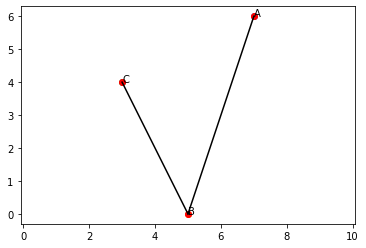
\includegraphics[width=\columnwidth]{Assignment1.png}
    \caption{Plot representing the Points}
    \label{Fig.1}
\end{figure}
\end{document}
